\documentclass{article}
\usepackage{tikz}
\usepackage{pgfplots}
\usepackage{textcomp}
\usepackage{array}
\usepackage{tabu}
\usepackage{numprint}
\begin{document}
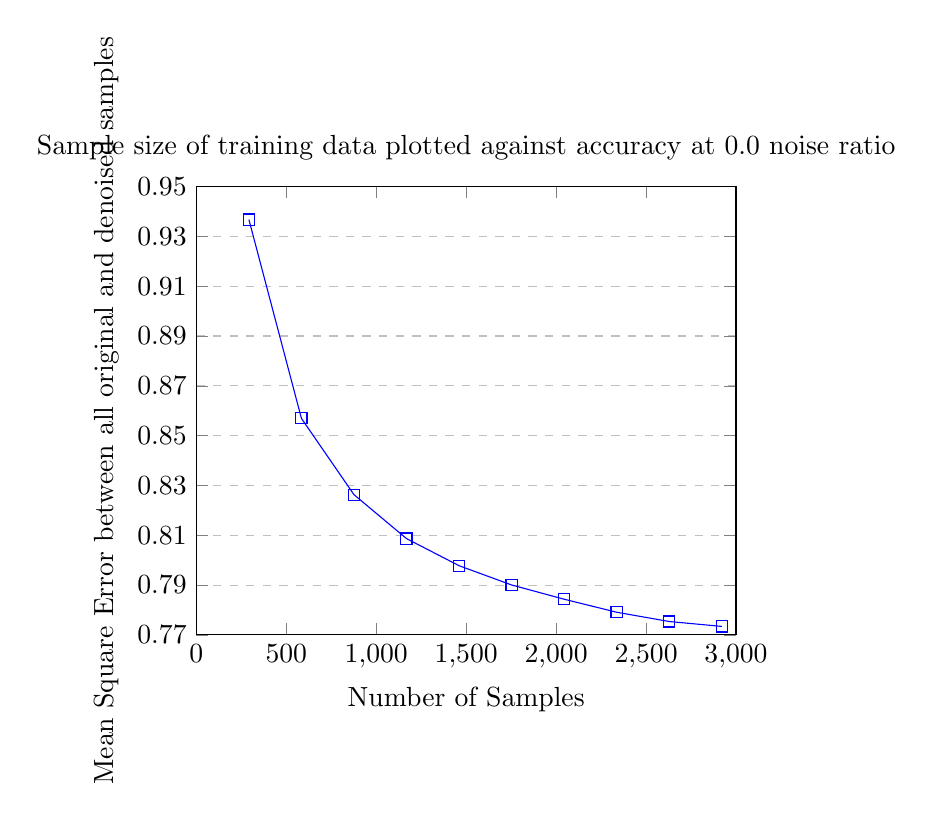
\begin{tikzpicture}
\begin{axis}[
title={Sample size of training data plotted against accuracy at 0.0 noise ratio},
xlabel={Number of Samples},
ylabel={Mean Square Error between all original and denoised samples},
xmin=0, xmax=3000,
ymin=0.77, ymax=0.95,
xtick={0,500,1000,1500,2000,2500,3000},
ytick={0.77, 0.79,0.81,0.83,0.85,0.87,0.89,0.91,0.93,0.95},
legend pos=north west,
ymajorgrids=true,
grid style=dashed,
]

\addplot[
color=blue,
mark=square,
]
coordinates {

(292, 0.9367609248325702)
(584, 0.856929376631142)
(876, 0.8263122200252626)
(1168, 0.8086658425021087)
(1460, 0.797795713386061)
(1752, 0.7900490169136227)
(2044, 0.784328546071565)
(2336, 0.7791018718090634)
(2628, 0.7753738005970627)
(2921, 0.7733999505156717)
    };
\end{axis}
\end{tikzpicture}

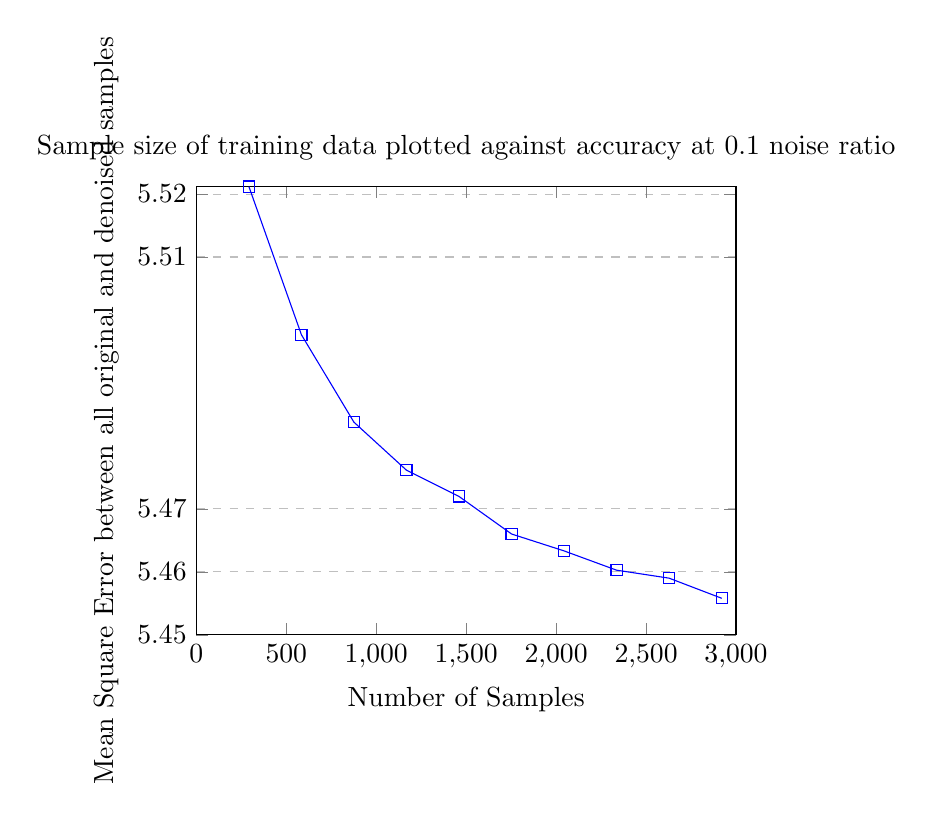
\begin{tikzpicture}
\begin{axis}[
title={Sample size of training data plotted against accuracy at 0.1 noise ratio},
xlabel={Number of Samples},
ylabel={Mean Square Error between all original and denoised samples},
xmin=0, xmax=3000,
ymin=5.45, ymax=5.521191432572333,
xtick={0,500,1000,1500,2000,2500,3000},
ytick={5.450,5.460,5.470,4.480,4.490,4.500,5.510,5.520,5.530},
legend pos=north west,
ymajorgrids=true,
grid style=dashed,
]

\addplot[
color=blue,
mark=square,
]
coordinates {

(292, 5.521191432572333)
(584, 5.497661751464459)
(876, 5.483775186651917)
(1168, 5.476152507625206)
(1460, 5.47198107080723)
(1752, 5.466023280863834)
(2044, 5.4633367043005485)
(2336, 5.460274007263241)
(2628, 5.45900741531701)
(2921, 5.455806780104275)
    };
\end{axis}
\end{tikzpicture}


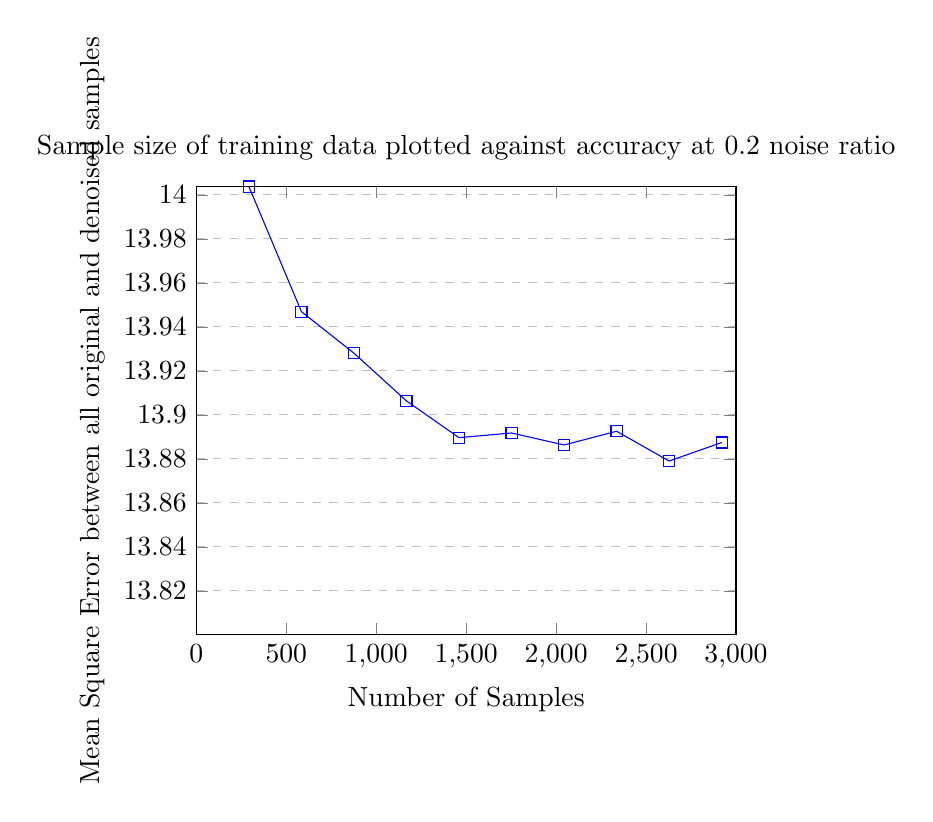
\begin{tikzpicture}
\begin{axis}[
title={Sample size of training data plotted against accuracy at 0.2 noise ratio},
xlabel={Number of Samples},
ylabel={Mean Square Error between all original and denoised samples},
xmin=0, xmax=3000,
ymin=13.80, ymax=14.003741996517524,
xtick={0,500,1000,1500,2000,2500,3000},
ytick={13.82,13.84,13.86,13.88,13.90,13.92,13.94,13.96,13.98,14.0},
legend pos=north west,
ymajorgrids=true,
grid style=dashed,
]

\addplot[
color=blue,
mark=square,
]
coordinates {

(292, 14.003741996517524)
(584, 13.946890303202288)
(876, 13.928029335277001)
(1168, 13.906324841449283)
(1460, 13.889636647464283)
(1752, 13.89175348641097)
(2044, 13.886305424275859)
(2336, 13.892547329329691)
(2628, 13.879008376745702)
(2921, 13.887434013725427)
    };
\end{axis}
\end{tikzpicture}

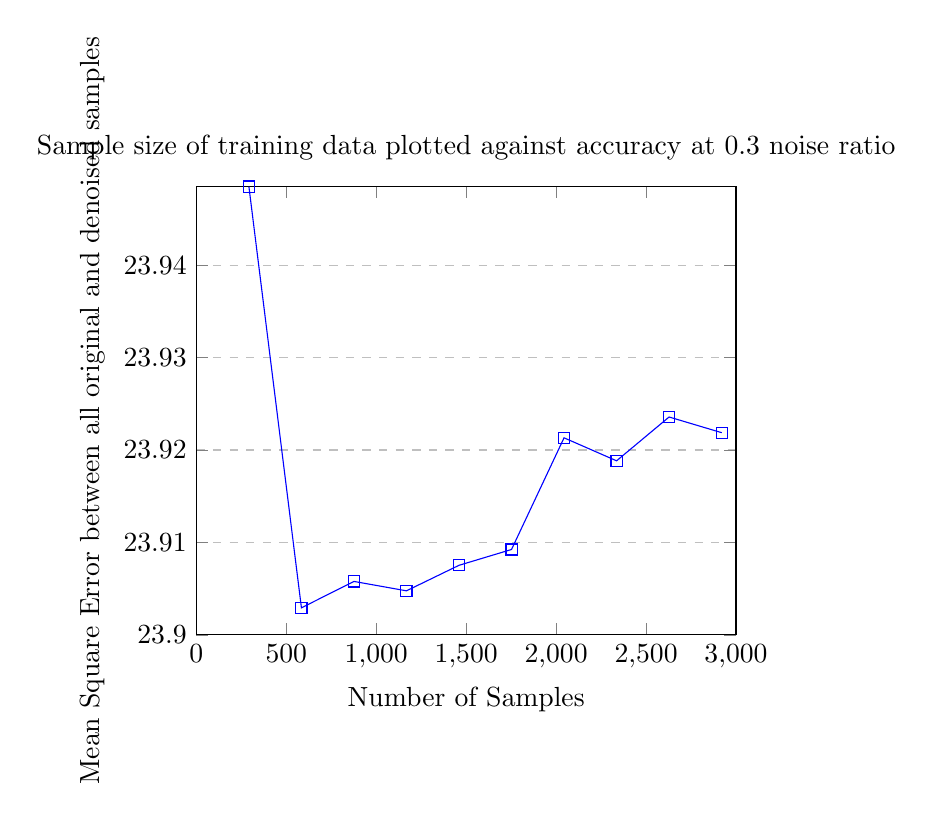
\begin{tikzpicture}
\begin{axis}[
title={Sample size of training data plotted against accuracy at 0.3 noise ratio},
xlabel={Number of Samples},
ylabel={Mean Square Error between all original and denoised samples},
xmin=0, xmax=3000,
ymin=23.90, ymax=23.94850078680391,
xtick={0,500,1000,1500,2000,2500,3000},
ytick={23.90,23.910,23.920,23.930,23.940,23.950},
legend pos=north west,
ymajorgrids=true,
grid style=dashed,
]

\addplot[
color=blue,
mark=square,
]
coordinates {

(292, 23.94850078680391)
(584, 23.902927171482254)
(876, 23.905783087696324)
(1168, 23.904766743252612)
(1460, 23.907527644713475)
(1752, 23.90923866249551)
(2044, 23.921318059491135)
(2336, 23.918832623260684)
(2628, 23.92357243144446)
(2921, 23.921871318865087)
    };
\end{axis}
\end{tikzpicture}


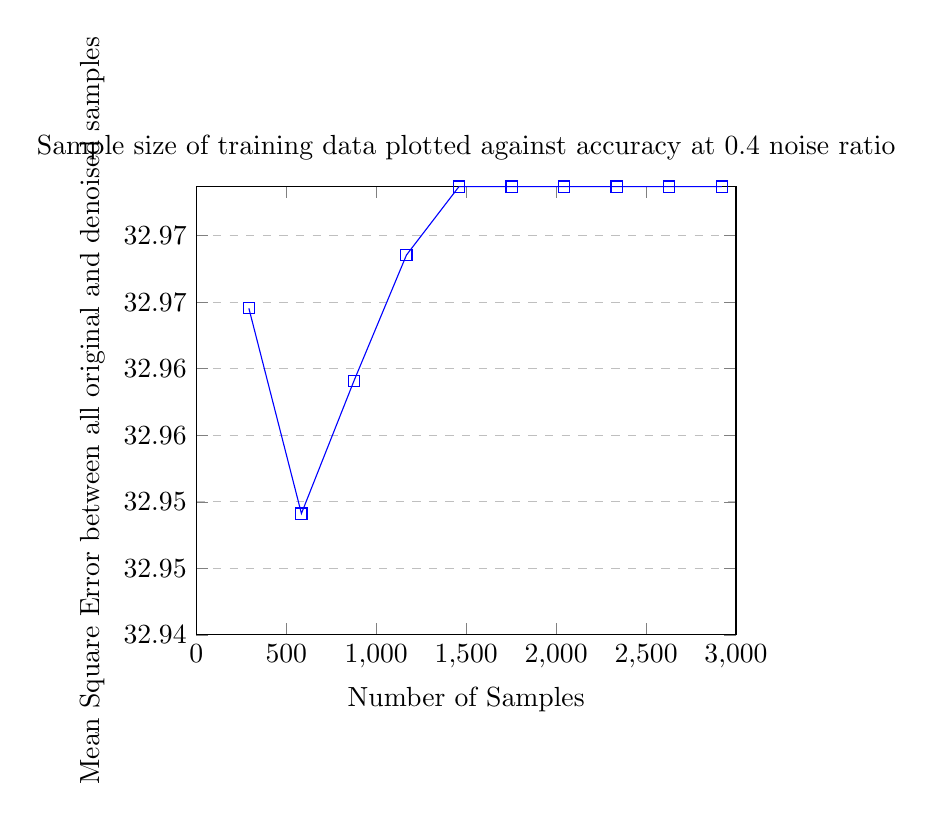
\begin{tikzpicture}
\begin{axis}[
title={Sample size of training data plotted against accuracy at 0.4 noise ratio},
xlabel={Number of Samples},
ylabel={Mean Square Error between all original and denoised samples},
xmin=0, xmax=3000,
ymin=32.94, ymax=32.97369393210016,
xtick={0,500,1000,1500,2000,2500,3000},
ytick={32.94, 32.945, 32.950, 32.955,32.960,32.965,32.970,32.975},
legend pos=north west,
ymajorgrids=true,
grid style=dashed,
]

\addplot[
color=blue,
mark=square,
]
coordinates {

(292, 32.964538654634474)
(584, 32.94911985254299)
(876, 32.959088130215)
(1168, 32.968548510005036)
(1460, 32.97369393210016)
(1752, 32.97369393195391)
(2044, 32.9736939319416)
(2336, 32.97369393193754)
(2628, 32.973693931937134)
(2921, 32.97369393193857)
    };
\end{axis}
\end{tikzpicture}

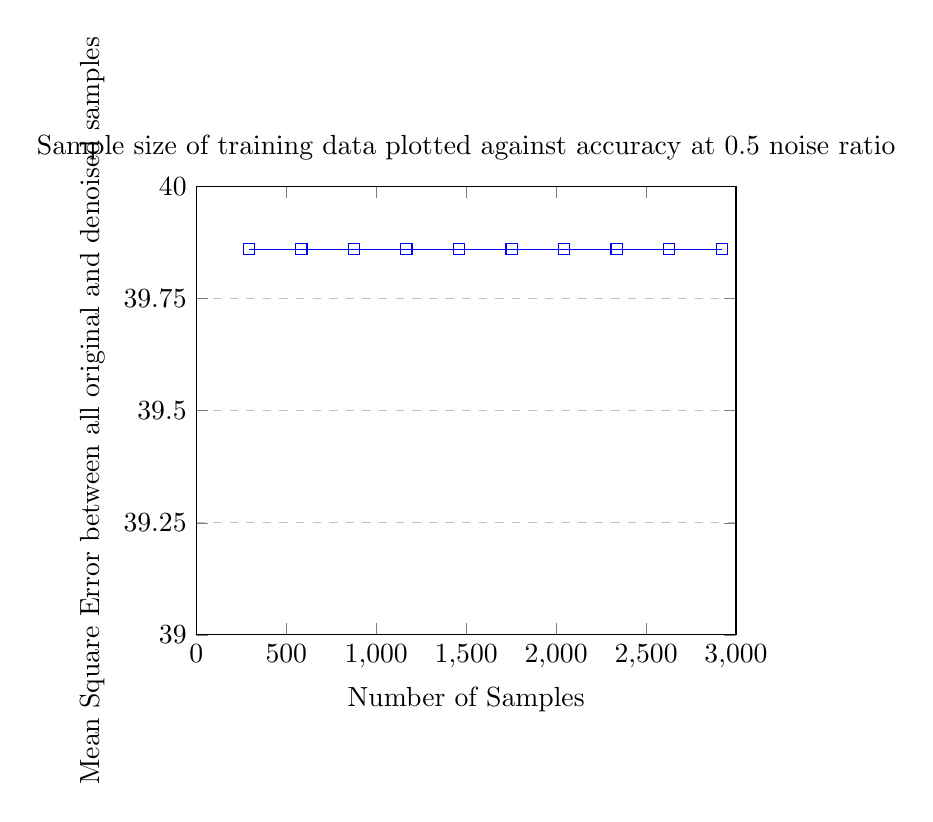
\begin{tikzpicture}
\begin{axis}[
title={Sample size of training data plotted against accuracy at 0.5 noise ratio},
xlabel={Number of Samples},
ylabel={Mean Square Error between all original and denoised samples},
xmin=0, xmax=3000,
ymin=39, ymax=40,
xtick={0,500,1000,1500,2000,2500,3000},
ytick={39, 39.25,39.5,39.75,40},
legend pos=north west,
ymajorgrids=true,
grid style=dashed,
]

\addplot[
color=blue,
mark=square,
]
coordinates {

(292, 39.859971985712825)
(584, 39.859971985712825)
(876, 39.859971985712825)
(1168, 39.859971985712825)
(1460, 39.859971985712825)
(1752, 39.859971985712825)
(2044, 39.859971985712825)
(2336, 39.859971985712825)
(2628, 39.859971985712825)
(2921, 39.859971985712825)
    };
\end{axis}
\end{tikzpicture}


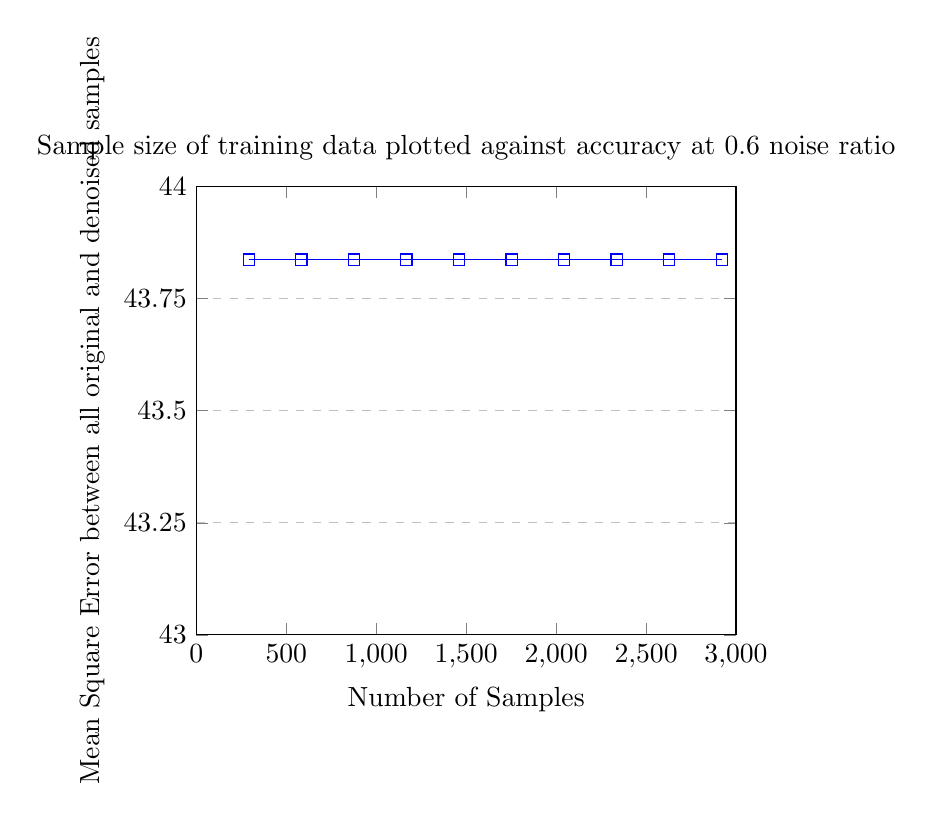
\begin{tikzpicture}
\begin{axis}[
title={Sample size of training data plotted against accuracy at 0.6 noise ratio},
xlabel={Number of Samples},
ylabel={Mean Square Error between all original and denoised samples},
xmin=0, xmax=3000,
ymin=43, ymax=44,
xtick={0,500,1000,1500,2000,2500,3000},
ytick={43,43.25,43.5,43.75,44},
legend pos=north west,
ymajorgrids=true,
grid style=dashed,
]

\addplot[
color=blue,
mark=square,
]
coordinates {

(292, 43.83718095731962)
(584, 43.83718095731962)
(876, 43.83718095731962)
(1168, 43.83718095731962)
(1460, 43.83718095731962)
(1752, 43.83718095731962)
(2044, 43.83718095731962)
(2336, 43.83718095731962)
(2628, 43.83718095731962)
(2921, 43.83718095731962)
    };
\end{axis}
\end{tikzpicture}


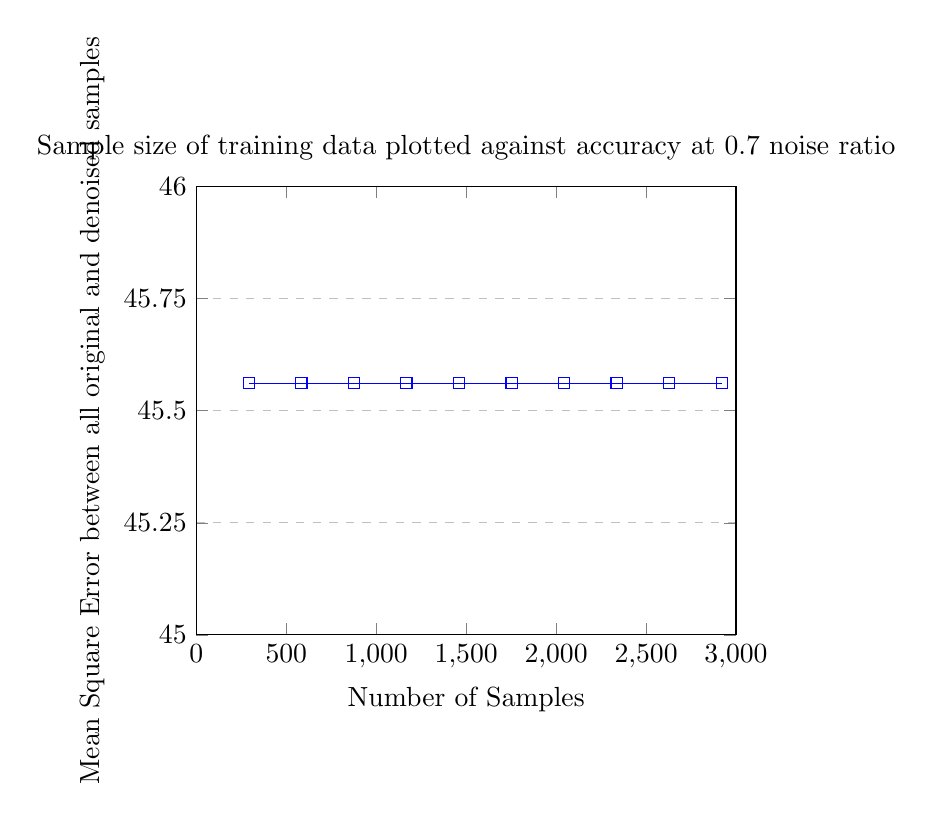
\begin{tikzpicture}
\begin{axis}[
title={Sample size of training data plotted against accuracy at 0.7 noise ratio},
xlabel={Number of Samples},
ylabel={Mean Square Error between all original and denoised samples},
xmin=0, xmax=3000,
ymin=45, ymax=46,
xtick={0,500,1000,1500,2000,2500,3000},
ytick={45,45.25,45.5,45.75,46},
legend pos=north west,
ymajorgrids=true,
grid style=dashed,
]

\addplot[
color=blue,
mark=square,
]
coordinates {

(292, 45.56126934688987)
(584, 45.56126934688987)
(876, 45.56126934688987)
(1168, 45.56126934688987)
(1460, 45.56126934688987)
(1752, 45.56126934688987)
(2044, 45.56126934688987)
(2336, 45.56126934688987)
(2628, 45.56126934688987)
(2921, 45.56126934688987)
    };
\end{axis}
\end{tikzpicture}


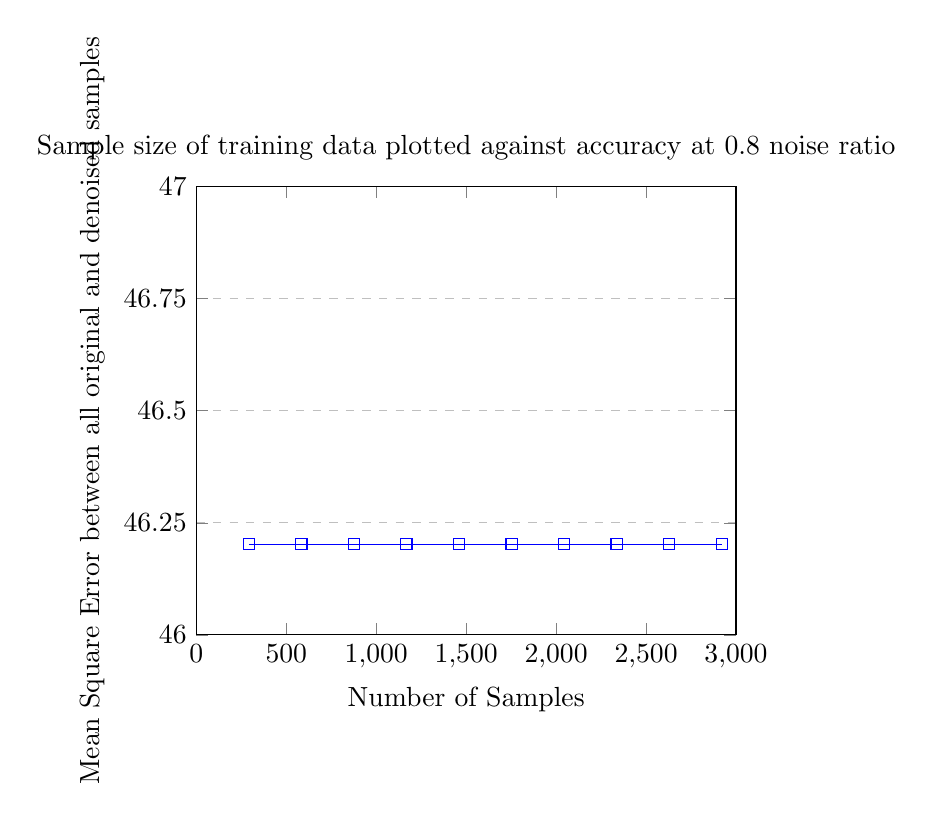
\begin{tikzpicture}
\begin{axis}[
title={Sample size of training data plotted against accuracy at 0.8 noise ratio},
xlabel={Number of Samples},
ylabel={Mean Square Error between all original and denoised samples},
xmin=0, xmax=3000,
ymin=46, ymax=47,
xtick={0,500,1000,1500,2000,2500,3000},
ytick={46,46.25,46.5,46.75,47},
legend pos=north west,
ymajorgrids=true,
grid style=dashed,
]

\addplot[
color=blue,
mark=square,
]
coordinates {

(292, 46.20184219579645)
(584, 46.20184219579645)
(876, 46.20184219579645)
(1168, 46.20184219579645)
(1460, 46.20184219579645)
(1752, 46.20184219579645)
(2044, 46.20184219579645)
(2336, 46.20184219579645)
(2628, 46.20184219579645)
(2921, 46.20184219579645)
    };
\end{axis}
\end{tikzpicture}


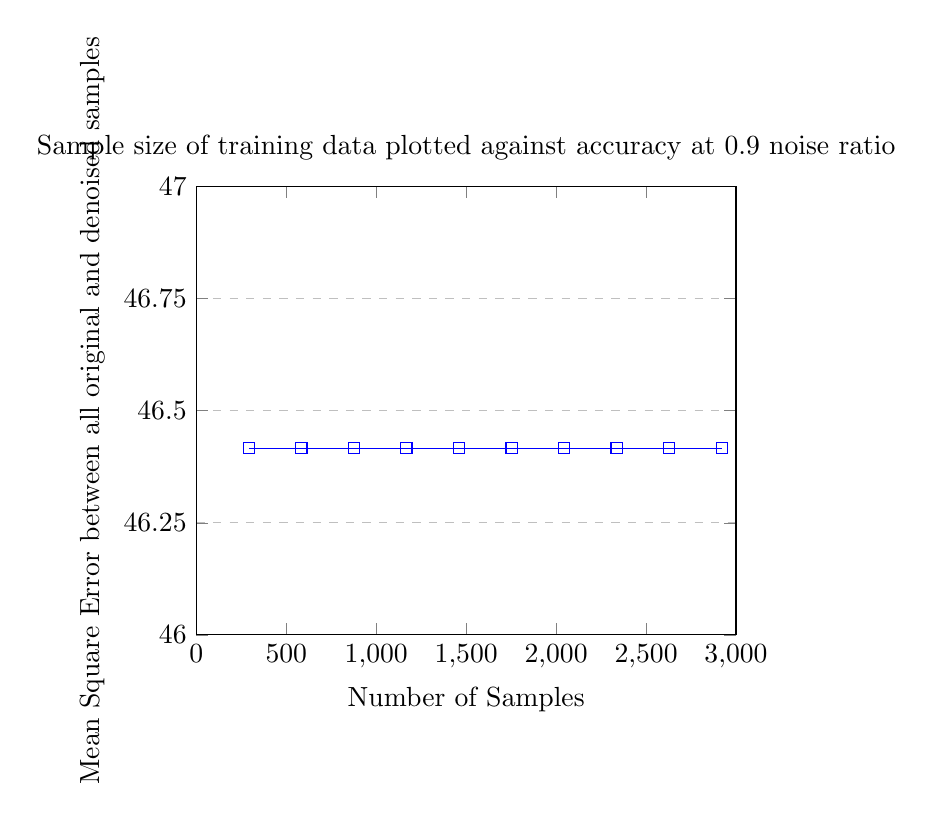
\begin{tikzpicture}
\begin{axis}[
title={Sample size of training data plotted against accuracy at 0.9 noise ratio},
xlabel={Number of Samples},
ylabel={Mean Square Error between all original and denoised samples},
xmin=0, xmax=3000,
ymin=46, ymax=47,
xtick={0,500,1000,1500,2000,2500,3000},
ytick={46,46.25,46.5,46.75,47},
legend pos=north west,
ymajorgrids=true,
grid style=dashed,
]

\addplot[
color=blue,
mark=square,
]
coordinates {

(292, 46.41662836680372)
(584, 46.41662836680372)
(876, 46.41662836680372)
(1168, 46.41662836680372)
(1460, 46.41662836680372)
(1752, 46.41662836680372)
(2044, 46.41662836680372)
(2336, 46.41662836680372)
(2628, 46.41662836680372)
(2921, 46.41662836680372)
    };
\end{axis}
\end{tikzpicture}

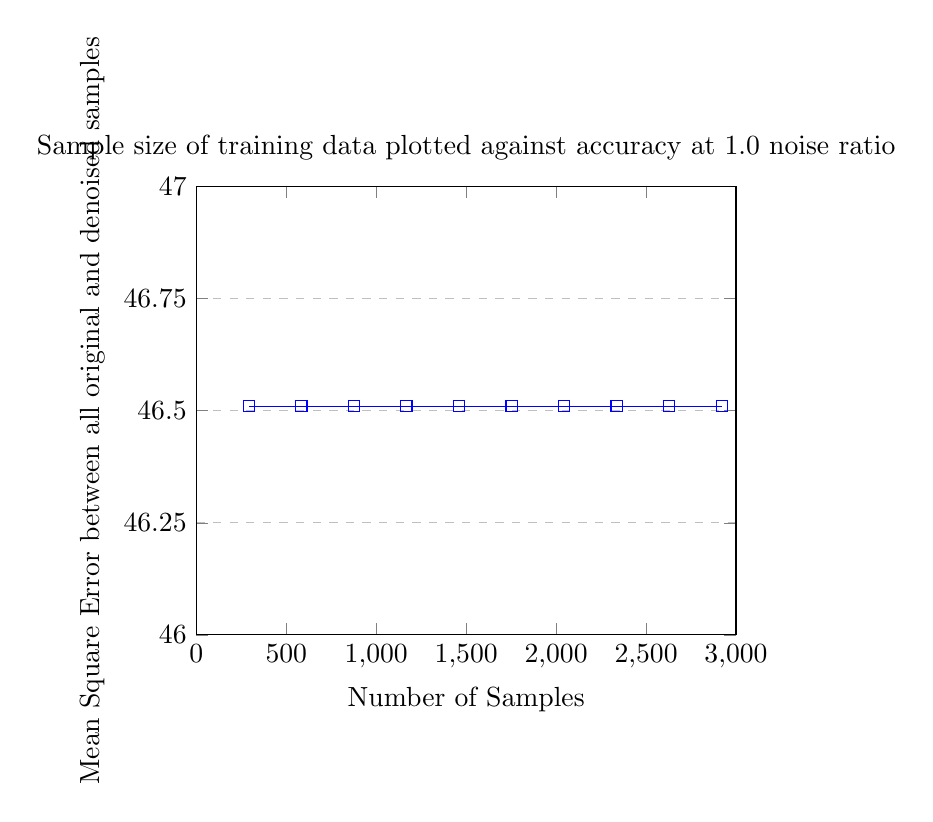
\begin{tikzpicture}
\begin{axis}[
title={Sample size of training data plotted against accuracy at 1.0 noise ratio},
xlabel={Number of Samples},
ylabel={Mean Square Error between all original and denoised samples},
xmin=0, xmax=3000,
ymin=46, ymax=47,
xtick={0,500,1000,1500,2000,2500,3000},
ytick={46,46.25,46.5,46.75,47},
legend pos=north west,
ymajorgrids=true,
grid style=dashed,
]

\addplot[
color=blue,
mark=square,
]
coordinates {

(292, 46.51019392874517)
(584, 46.51019392874517)
(876, 46.51019392874517)
(1168, 46.51019392874517)
(1460, 46.51019392874517)
(1752, 46.51019392874517)
(2044, 46.51019392874517)
(2336, 46.51019392874517)
(2628, 46.51019392874517)
(2921, 46.51019392874517)
    };
\end{axis}
\end{tikzpicture}






\end{document}